\documentclass[aspectratio=169]{beamer}
   \usetheme{metropolis}
   \setbeamertemplate{blocks}[rounded][shadow=false]
\usepackage{url}
\usepackage{hyperref}
\usepackage{booktabs}
\usepackage{tabularx}
\usepackage{dcolumn}
   \newcolumntype{d}[1]{D{.}{.}{#1}}
\usepackage{graphicx}
\usepackage{listings}
\usepackage{adjustbox}
\usepackage{color}
\usepackage{textpos}
\usepackage{etoolbox}

\makeatletter
\patchcmd{\beamer@sectionintoc}{\vskip1.5em}{\vskip0.5em}{}{}
\makeatother

\definecolor{smured}{rgb}{0.797,0,0.027}
\definecolor{smublue}{RGB}{48,64,116}
\definecolor{dkgreen}{rgb}{0,0.6,0}
\definecolor{gray}{rgb}{0.5,0.5,0.5}
\definecolor{mauve}{rgb}{0.58,0,0.82}
\definecolor{text_gray}{RGB}{46,58,62}

\setbeamercolor{progress bar}{fg=smured,bg=smublue}
\setbeamercolor{title separator}{fg=smublue}
\setbeamercolor{frametitle}{bg=smublue}

\metroset{
  numbering=fraction
}

\hypersetup{
  colorlinks=true,
  allcolors=text_gray,
  urlcolor=smured,
}

\lstset{
  aboveskip=3mm,
  belowskip=3mm,
  showstringspaces=false,
  columns=flexible,
  basicstyle={\small\ttfamily},
  numbers=left,
  numberstyle=\tiny\color{gray},
  keywordstyle=\color{blue},
  commentstyle=\color{dkgreen},
  stringstyle=\color{mauve},
  breaklines=false,
  breakatwhitespace=true,
  tabsize=3
}

\addtobeamertemplate{frametitle}{}{
\begin{textblock*}{1cm}(\textwidth,-1.155cm)

\includegraphics[width=1cm]{figures/smu_logo.pdf}
\end{textblock*}}

\title[oneAPI]{Intel oneAPI HPC Toolkit Overview}
\author{Robert Kalescky\\ HPC Applications Scientist}
\institute{
Research and Data Sciences Services\\
Office of Information Technology\\
Center for Research Computing\\
Southern Methodist University}
\date{March 10, 2021}

\begin{document}

\begin{frame}
\titlepage
\end{frame}

\begin{frame}{Outline}
\footnotesize
\tableofcontents[hideallsubsections]
\end{frame}

\section{Research Support}

\begin{frame}{Research and Data Science Services}
\begin{itemize}
  \item Provide research computing support, consultations, and collaborations
  \item Data Science - Dr. Eric Godat
  \item High-Performance Computing - Dr. Robert Kalescky \& Dr. John LaGrone
  \item Custom Devices (IOT, wearables, etc.) - Guillermo Vasquez
\end{itemize}
\end{frame}

\begin{frame}{Center for Research Computing (CRC)}
\begin{itemize}
  \item Maintains our primary shared resource for research computing, ManeFrame II (M2), in collaboration with OIT
  \item Provides research computing tools, support, and training to all faculty, staff, and students using research computing resources
  \item \url{www.smu.edu/crc} has documentation and news
  \item \href{mailto:help@smu.edu}{help@smu.edu} or \href{mailto:rkalescky@smu.edu}{rkalescky@smu.edu} for help
  \item Request an account at \url{www.smu.edu/crc}
\end{itemize}
\end{frame}

\begin{frame}{Spring 2022 CRC HPC Workshop Series}
\begin{table}
\tiny
\begin{tabular}{lll}
Date     & Time  & Workshop\\
\hline
February 2 & 2-4 & ManeFrame II (M2) Introduction \\  
February 9 & 2-4 & Workflows in R \\  
February 15 & 3-5 & Finding and Preparing Text Data Sets for Mining \\
Febryary 16 & 1-4 & Machine Learning with Python Part 1 \\
February 17 & 12-1 & AI for the Non-Expert \\
February 18 & 12-1 & Introduction to GitHub \\        
February 23 & 2-4  & Containers and Spack \\     
March 2   &  2-4 &  ManeFrame II (M2) Introduction \\
March 3   &  1-4 & Data Science Workflow with R \\  
March 8   &  3-6 & Introduction to Python for Text Mining \\ 
March 9   &  1-4 & Machine Learning with Python Part 2 \\ 
March 22  &  3-6 & Getting Support for Text Mining \\  
March 23  &  2-4 & Shared Memory Parallelism \\   
March 30  &  1-4 & Deep Learning with Python Part 1 \\   
April 6   &  2-4 & ManeFrame II (M2) Introduction \\    
April 13  &  2-4 & Accelerator Libraries and APIs \\    
April 20  &  1-4 & Deep Learning with Python Part 2 \\      
April 27  &  2-4 & MPI/NCCL/SHMem \\            
May 4     &  2-4 & ManeFrame II (M2) Introduction      
\end{tabular}
\caption{Workshops will be held each Wednesday from 2:00 to 4:00 PM. Sessions will typically be                                
recorded and posted along with session materials.         
Register on the Library Workshop Calendar \href{https://libcal.smu.edu/calendar/libraryworkshops}{https://libcal.smu.edu/calendar/libraryworkshops}
}
\end{table}
\end{frame}

\section{ManeFrame II (M2)}

\begin{frame}{Cluster Super Computers}
\begin{figure}
  \centering
  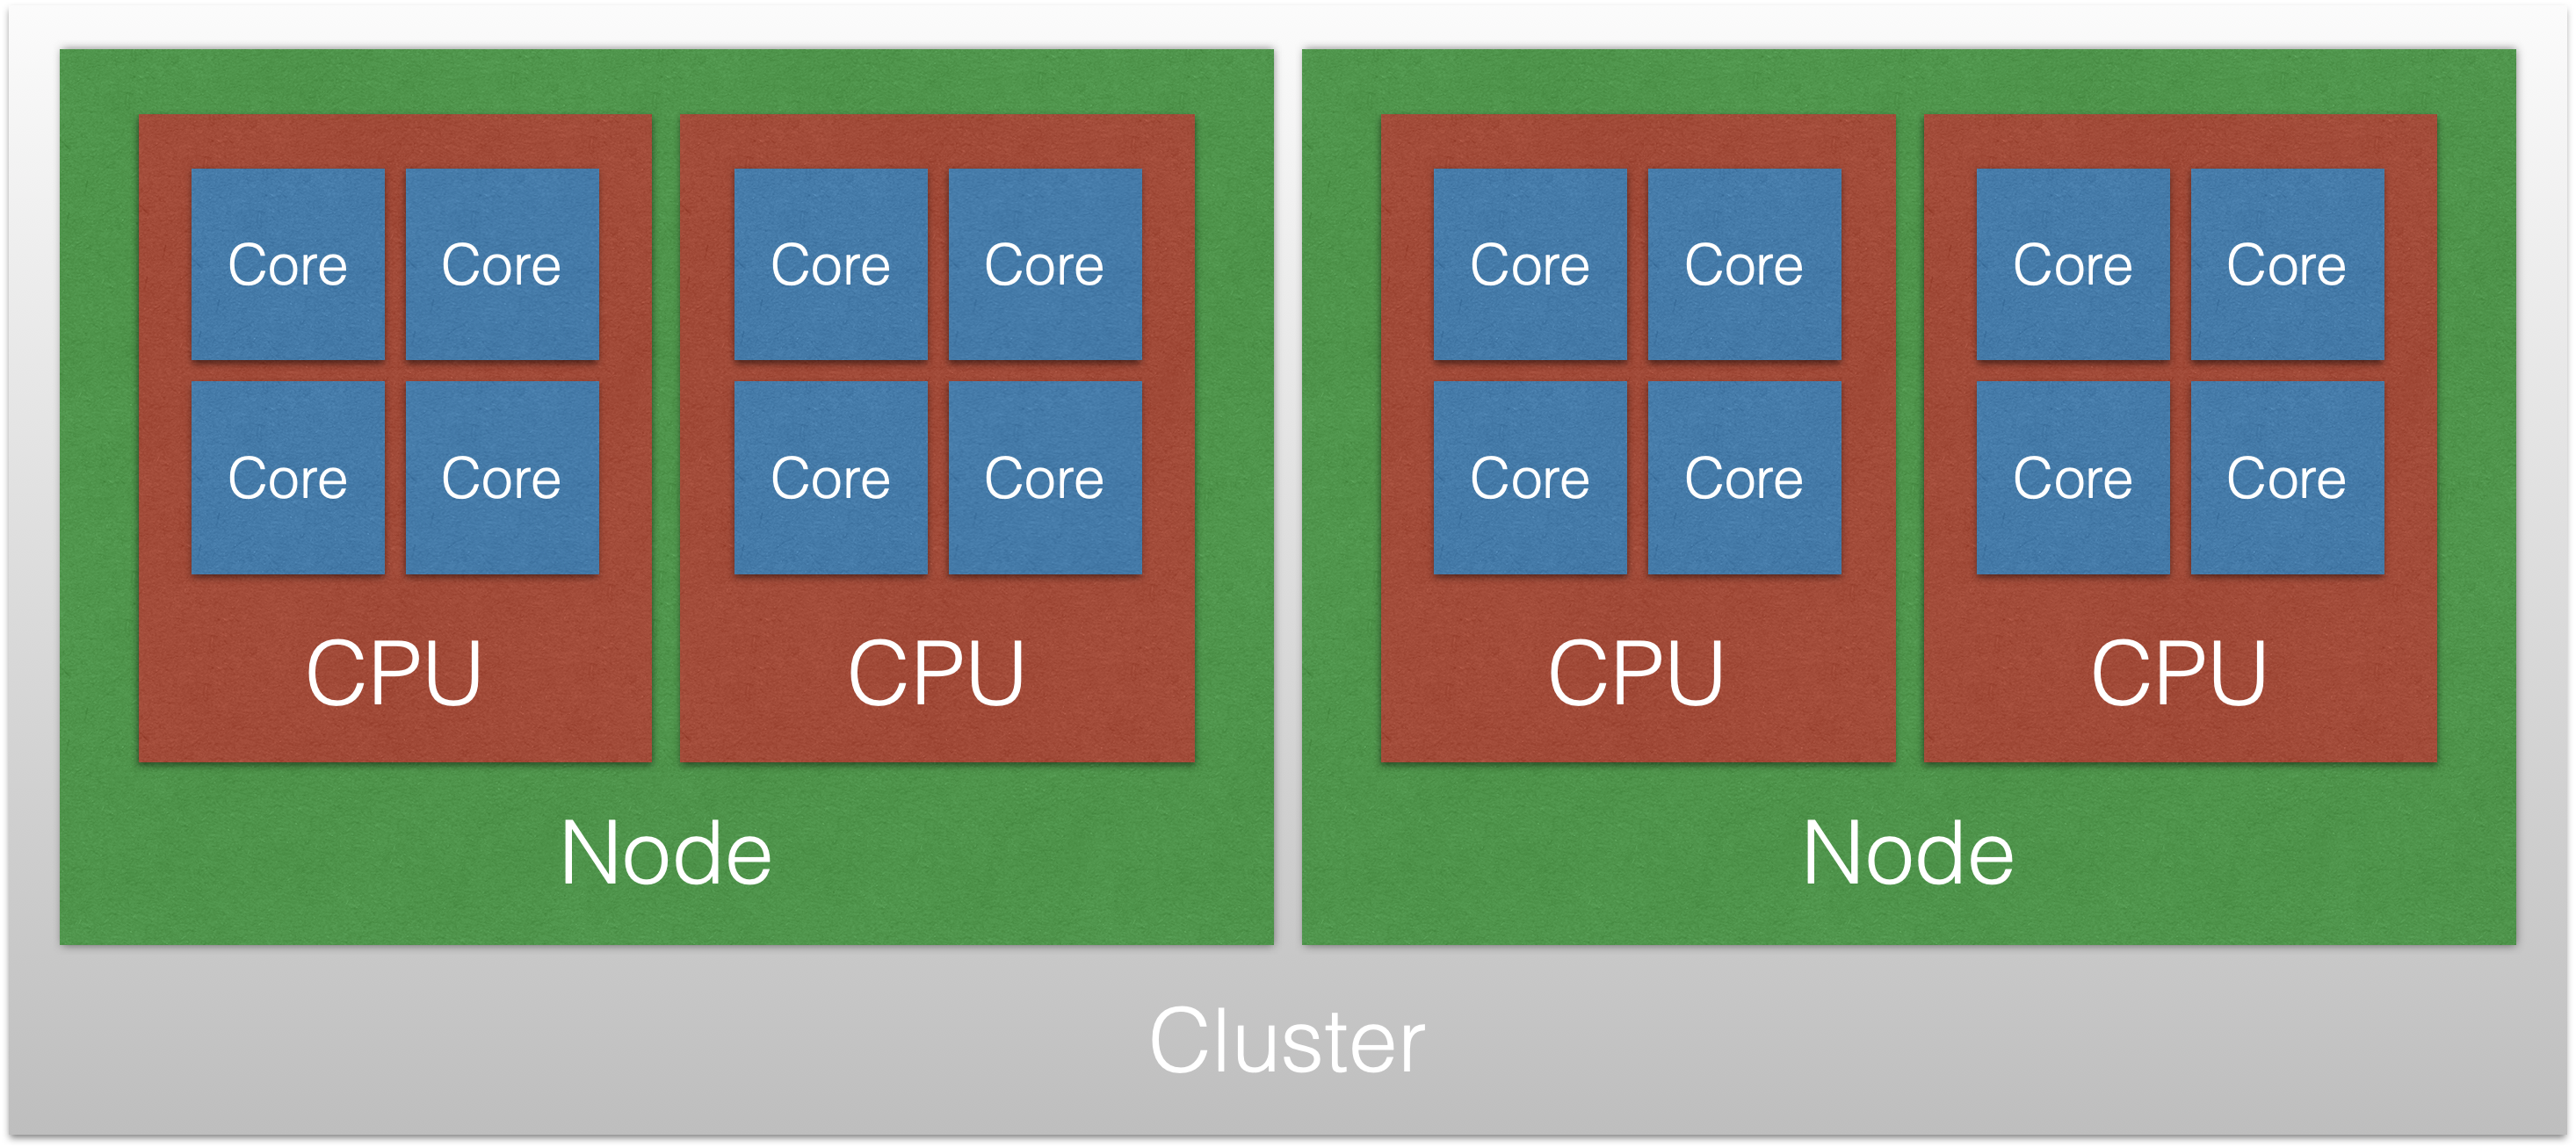
\includegraphics[width=0.75\linewidth]{figures/cluster.png}
  \caption{A cluster is a collection of individual computers networked together. Applications can be configured to run on all available compute resources.}
\end{figure}
\end{frame}

\begin{frame}{ManeFrame II (M2) Node Types}
\begin{table}
\tiny
\begin{tabular}{lllll}
\toprule
Type & Quantity & Cores & Memory [GB] & Additional Resources\\
\midrule
Standard-Memory & 176 & 36 & 256 & \\
Medium-Memory-1 & 35 & 36 & 768 & \\
Medium-Memory-2 & 4 & 24 & 768 & 3 TB SSD local scratch\\
High-Memory-1 & 5 & 36 & 1,536 & \\
High-Memory-2 & 6 & 40 & 1,536 & 3 TB SSD local scratch\\
GPGPU-1 & 36 & 36 & 256 & NVIDIA P100 GPU has 3,584 CUDA cores and 16 GB CoWoS\\
MIC-1 & 36 & 64 & 384 & 16 GB of high bandwidth (400 GB/s) stacked memory\\
VDI & 5 & 36 & 256 & NVIDIA Quadro M5000 GPU\\
v100x8 & 3 & 36 & 768 & 8 NVIDIA V100 GPUs with 5,120 CUDA cores and 32 GB CoWoS\\
Faculty Partner Nodes & 3 &  &  & Various research specific NVIDIA GPU configurations\\
\midrule
ManeFrame II & 354 & 11,276 & 120 TB & 2.8 PB storage and InfiniBand network\\
\bottomrule
\end{tabular}
\end{table}
\end{frame}

\begin{frame}{ManeFrame II (M2) Partitions (Queues)}
\begin{table}
\tiny
\begin{tabular}{llll}
\toprule
Partition & Duration & Cores & Memory [GB]\\
\midrule
development & 2 hours & various & various\\
htc & 1 day & 1 & 6\\
standard-mem-s & 1 day & 36 & 256\\
standard-mem-m & 1 week & 36 & 256\\
standard-mem-l & 1 month & 36 & 256\\
medium-mem-1-s & 1 day & 36 & 768\\
medium-mem-1-m & 1 week & 36 & 768\\
medium-mem-1-l & 1 month & 36 & 768\\
medium-mem-2 & 2 weeks & 24 & 768\\
high-mem-1 & 2 weeks & 36 & 1538\\
high-mem-2 & 2 weeks & 40 & 1538\\
mic & 1 week & 64 & 384\\
gpgpu-1 & 1 week & 36 & 256\\
v100x8 & 1 week & 1 & 20\\
fp-gpgpu-2 & various & 24 & 128\\
fp-gpgpu-3 & various & 40 & 384\\
\bottomrule
\end{tabular}
\end{table}
\end{frame}

\begin{frame}{ManeFrame II File Systems}
\begin{description}
\item[\$HOME]
\begin{itemize}
  \item Default file system when logging into M2, e.g. \mintinline{sh}{/users/$USER}.
  \item Space should be used to write, edit, compile programs, and job submission scripts, etc.
  \item Restricted by quotas (200 GB) and backed-up.
\end{itemize}
\item[\$WORK]
\begin{itemize}
  \item Long term storage at \mintinline{sh}{/work/users/$USER}.
  \item Restricted by quotas (8 TB) and not backed-up.
\end{itemize}
\item[\$SCRATCH]
\begin{itemize}
 \item Scratch space at \mintinline{sh}{/scratch/users/$USER}.
 \item Treat \$SCRATCH as a volatile file system that is not backed-up.
 \item Beginning October 1, 2021, \mintinline{sh}{$SCRATCH} has a 60-day retention policy, i.e. untouched files will be removed after 60 days.
\end{itemize}
\end{description}
\end{frame}



\section{Using oneAPI On ManeFrame II (M2)}

\begin{frame}{Using oneAPI On ManeFrame II (M2)}
\begin{itemize}
  \item All Intel oneAPI compilers, libraries, and tools are made availabe on M2 via \lstinline{module load intel/oneAPI-2021.lua}
  \item \href{https://github.com/oneapi-src/oneAPI-samples}{Intel oneAPI Toolkit Samples}
\end{itemize}
\end{frame}

\begin{frame}{Components}
\begin{figure}
  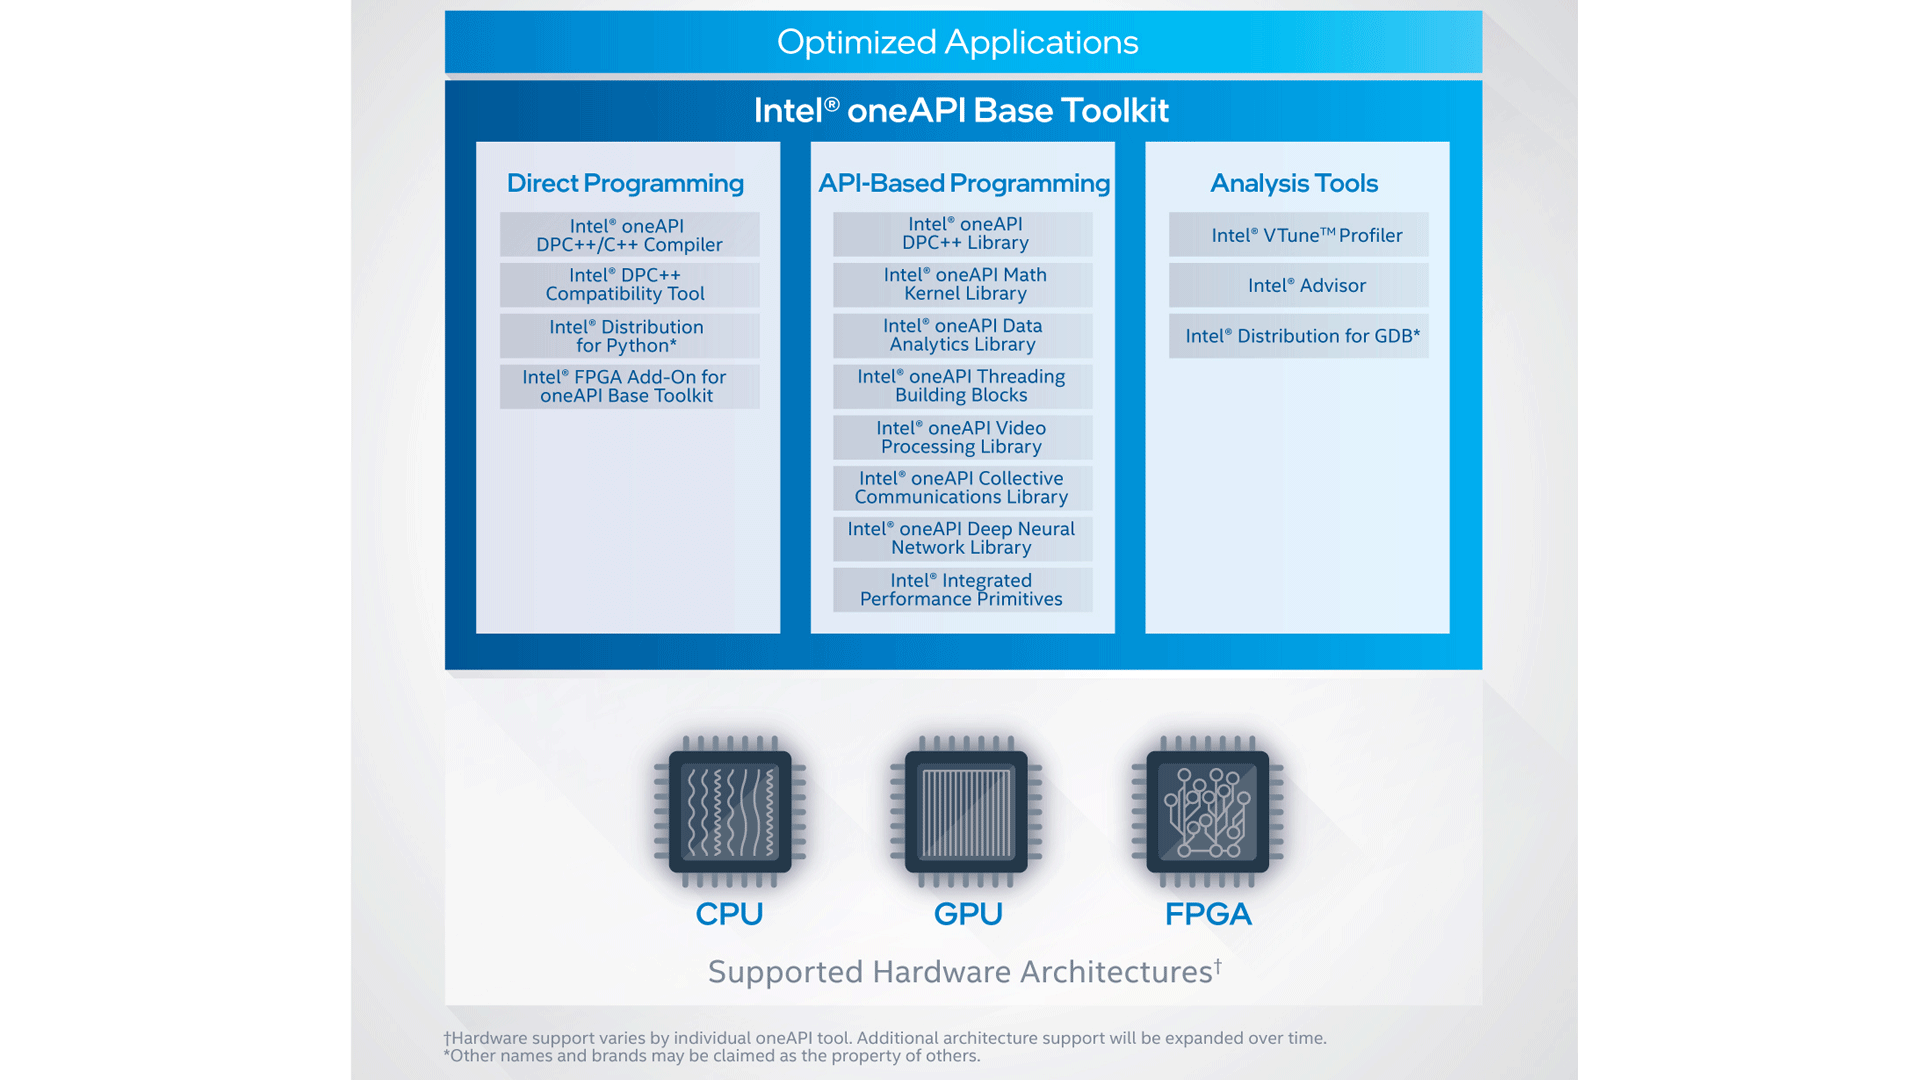
\includegraphics[width=0.75\linewidth]{figures/diagram-onapi-base-toolkit-16x9.png}
  \caption{Components of the oneAPI 2021 base installation.}
\end{figure}
\end{frame}

\section{Compilers}

\begin{frame}{oneAPI DPC++/C++ Compiler}
\begin{columns}
\begin{column}{0.5\textwidth}
\begin{itemize}
  \item Standards-based C++ compiler based on the open source LLVM compiler infrastructure
  \begin{itemize}
    \item Full support up through C++17
    \item Initial support for C++20
  \end{itemize}
  \item SYCL compiler
  \item DPC++ compiler (SYCL with Intel extensions)
  \item Partial support for OpenMP 4.5 and 5.0 offloading
\end{itemize}
\end{column}
\begin{column}{0.5\textwidth}
\begin{figure}
  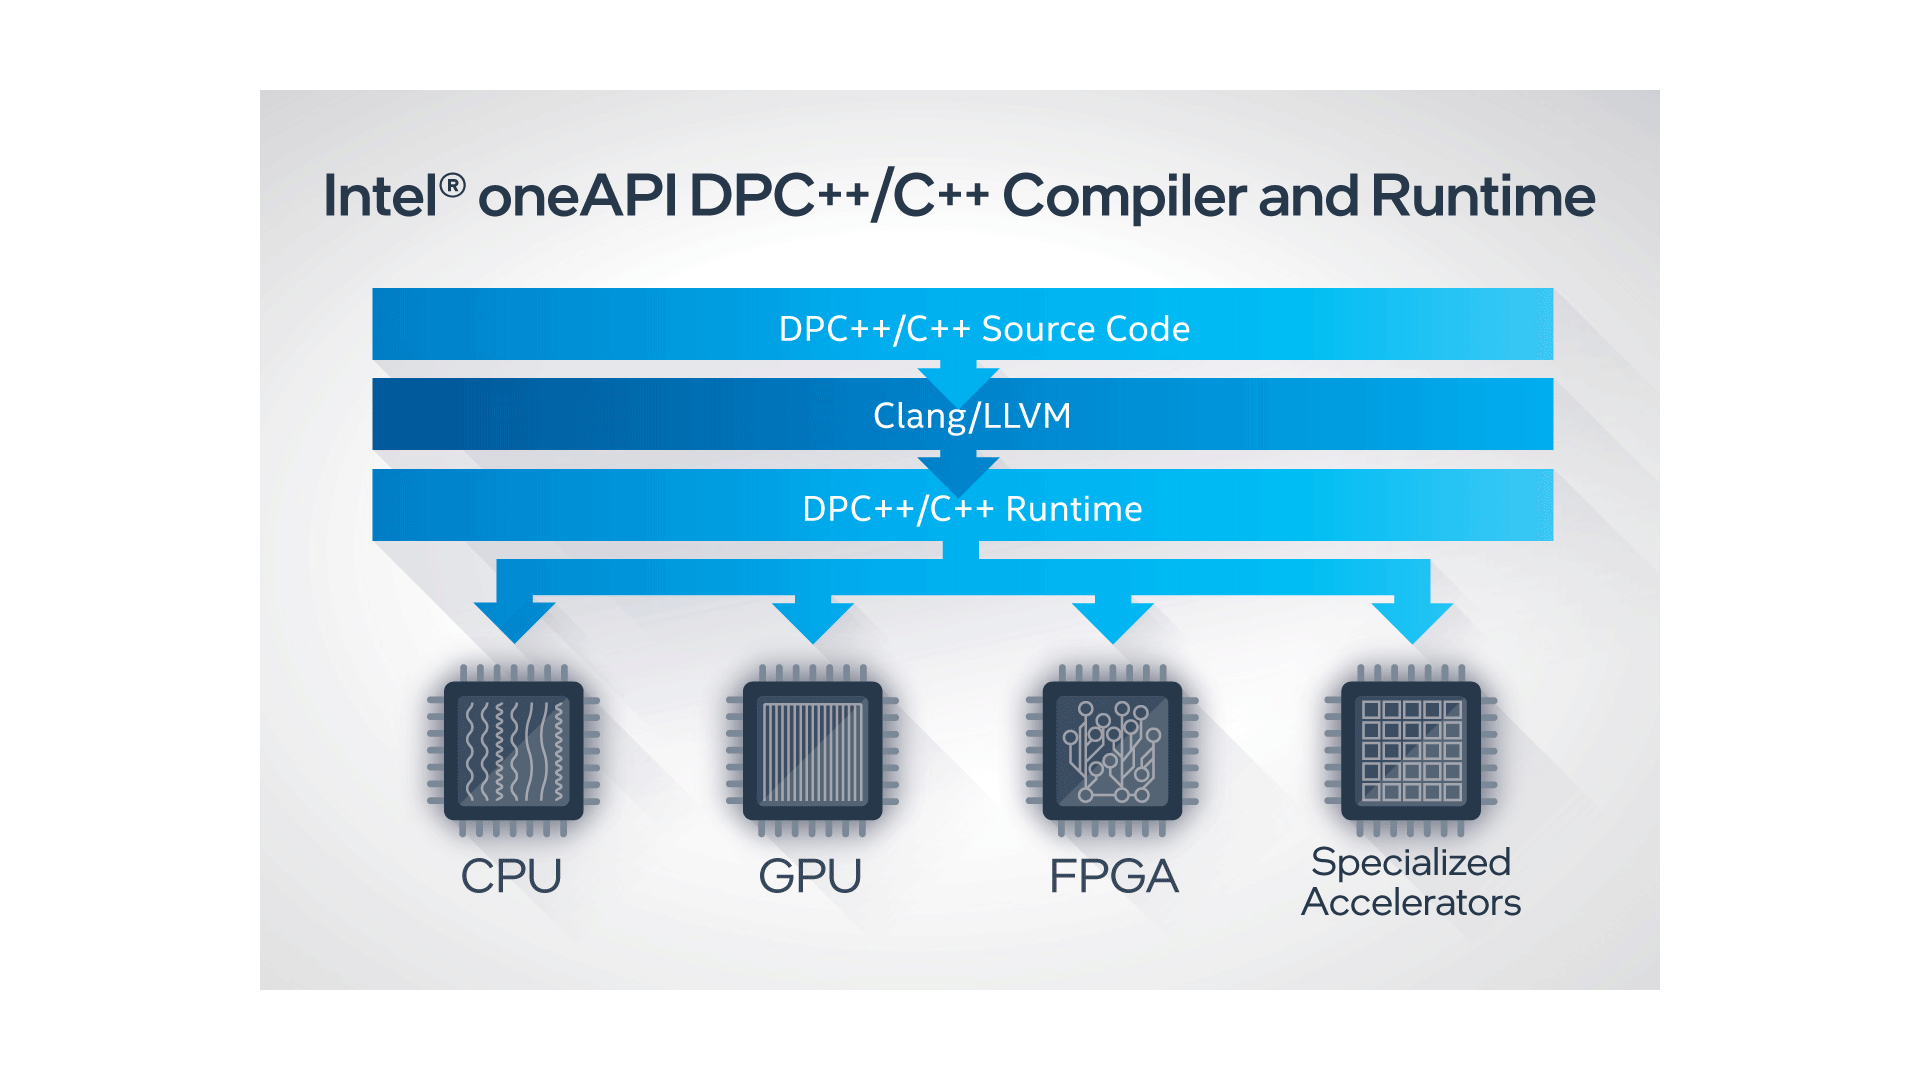
\includegraphics[width=\linewidth]{figures/diagram-oneapi-dpc-c-compiler-16x9.png}
  \caption{oneAPI DPC++ and C++ compiler and runtime.}
\end{figure}
\end{column}
\end{columns}
\end{frame}

\begin{frame}{Intel Fortran Compiler (Beta)}
\begin{itemize}
  \item Standards-based Fortran compiler based on the open-source LLVM compiler infrastructure
  \begin{itemize}
    \item Support for many Fortran standards
  \end{itemize}
  \item Automatic parallelism
  \item Coarray support
  \item Automatic processor dispatch
  \item Partial support for OpenMP 4.5 and 5.0 offloading
\end{itemize}
\end{frame}

\begin{frame}{Classic Compilers}
\begin{itemize}
  \item Provides continuity with previous line of Intel compilers
  \item Workings with existing workflows
  \item Updated for currently supported hardware
\end{itemize}
\end{frame}

\begin{frame}{Intel MPI Library}
\begin{itemize}
  \item Based on the open-source MPICH implementation
  \item Supports up to MPI 3.1 on multiple fabrics
  \item Fast messaging via the OpenFabrics Interface (OFI)
  \item Support for modern interconnects
  \item ABI compatibility with existing MPI-1 and MPI-2 applications
\end{itemize}
\end{frame}

\section{SYCL}

\begin{frame}{What is SYCL?}
\begin{itemize}
  \item An abstraction layer for writing single-source pure C++17 data-parallel code
  \item Portions of SYCL code can be offloaded various devices, e.g. CPUs, GPUs, and FPGAs
  \item Wide hardware support:
  \begin{itemize}
    \item Intel CPUs, GPUs, and FPGAs
    \item AMD CPUs and GPUs
    \item NVIDIA GPUs
    \item ARM CPUs
    \item Power CPUs
  \end{itemize}
\end{itemize}
\end{frame}

\begin{frame}{What is DPC++?}
\begin{itemize}
  \item DPC++ is SYCL with Intel-specific extensions
  \item Some of the extensions are included in the most recent SYCL standard
  \item As Intel's DPC++ compiler is open-source, there is growing hardward support:
  \begin{itemize}
    \item Intel CPUs, GPUs, and FPGAs
    \item AMD CPUs and GPUs
    \item NVIDIA GPUs
    \item ARM CPUs
    \item Power CPUs
  \end{itemize}
\end{itemize}
\end{frame}

\begin{frame}{Why is SYLC important?}
\begin{itemize}
  \item Leadership-class HPC systems are increasingly heterogenous
  \item Various CPU and GPU combinations
  \begin{itemize}
    \item Intel CPUs, GPUs, and FPGAs
    \item AMD CPUs and GPUs
    \item NVIDIA GPUs
    \item ARM CPUs
    \item Power CPUs
  \end{itemize}
\end{itemize}
\end{frame}

\section{Libraries}

\begin{frame}{oneAPI Math Kernel Library}
\begin{itemize}
  \item Optimized library for scientific computing
  \item Create performant science and engineering applications
  \item Includes BLAS, LAPACK, sparse solvers, fast Fourier transforms (FFT), random number generator functions (RNG), summary statistics, data fitting, and vector math
  \item Heavily optimize routines for current and future generations of Intel CPUs, GPUs, and other accelerators
  \item Seamless upgrade for previous users of the Intel Math Kernel Library (MKL)
  \item New support for DPC++
  \item C and Fortran OpenMP Intel GPU offload
\end{itemize}
\end{frame}

\begin{frame}{oneAPI DPC++ Library}
\begin{itemize}
  \item Productivity APIs for heterogeneous computing
  \item Optimized standards-based and familiar APIs:
  \begin{itemize}
    \item C++ STL
    \item Parallel STL (PSTL)
    \item Boost.Compute
    \item Standard SYCL
  \end{itemize}
  \item Custom iterators for parallel algorithms
  \item Use device and host containers to target GPUs and FPGAs or run your code across multi-node CPUs
\end{itemize}
\end{frame}

\begin{frame}{oneAPI Threading Building Blocks}
\begin{itemize}
  \item Simplifies the work of adding parallelism to complex applications
  \item Runtime library automatically maps logical parallelism onto threads, making more efficient use of node resources
  \item Scalable data-parallel programming
    \begin{itemize}
    \item Multiple threads to work on different parts of a collection
    \item Scales well to larger numbers of processors by dividing the collection into smaller pieces
    \item Program performance increases as processors and accelerators are added
  \end{itemize}
\end{itemize}
\end{frame}

\begin{frame}{oneAPI Collective Communications Library}
\begin{itemize}
  \item Commonly used collective operations found in deep learning and machine learning workloads
  \item Enables efficient implementations of collectives that are heavily used for neural network training, including all-gather, all-reduce, and reduce-scatter
  \item Asynchronous progress for compute communication overlap
  \item Dedication of one or more cores to ensure optimal network use
  \item Message prioritization, persistence, and out-of-order execution
  \item Collectives in low-precision data types
\end{itemize}
\end{frame}

\begin{frame}{oneAPI Data Analytics Library}
\begin{itemize}
  \item Highly tuned set of optimiztion and analytic functions
  \item Tuned for the specific instruction set, vector width, core count, and memory architecture of each resource
  \item Functions include:
  \begin{itemize}
    \item Correlation and variance-covariance functions
    \item Classification and regression functions
    \item Optimization solver functions
    \item Component analysis
  \end{itemize}
\end{itemize}
\end{frame}

\begin{frame}{oneAPI Deep Neural Network Library}
\begin{itemize}
  \item Improve performance of deep learning frameworks on Intel hardware
  \item Optimized primitive operations such as convolution and data reordering
  \item Support for reduce precision data types:
  \begin{itemize}
    \item 16- and 32-bit floating points
    \item bfloat16
    \item 8-bit integers
  \end{itemize}
\end{itemize}
\end{frame}

\begin{frame}{Integrated Performance Primitives}
\begin{itemize}
  \item Highly optimized set of domain-specific functions:
  \begin{itemize}
    \item Image processing
    \item Data compression
    \item Signal processing
    \item Cryptography
  \end{itemize}
\end{itemize}
\end{frame}

\section{Tools}

\begin{frame}{DPC++ Compatibility Tool}
\begin{columns}
\begin{column}{0.5\textwidth}
\begin{itemize}
  \item Assists in migrating your existing CUDA code to DPC++
  \item Ports both CUDA language kernels and library API calls
  \item Inline comments help porting and tuning the DPC++ code
\end{itemize}
\end{column}
\begin{column}{0.5\textwidth}
\begin{figure}
  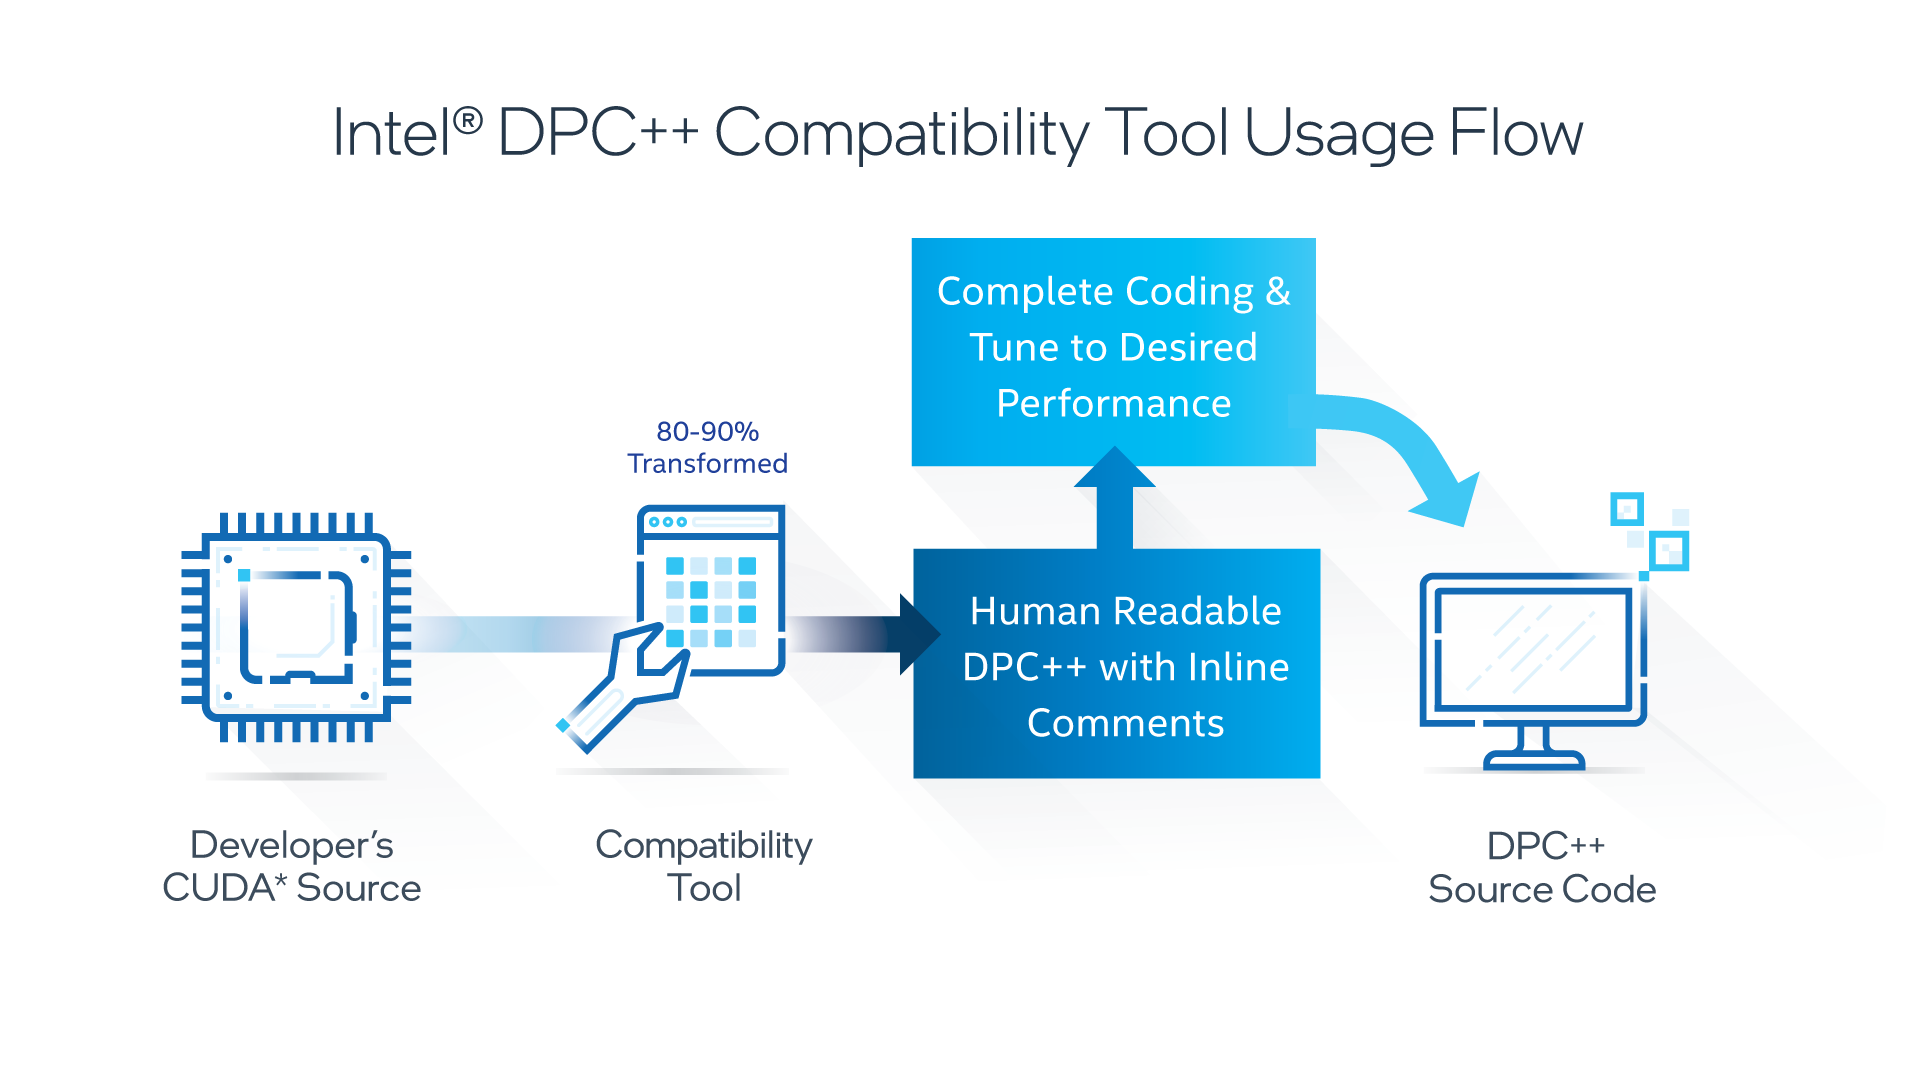
\includegraphics[width=\linewidth]{figures/diagram-oneapi-dpc-compat-tool-16x9.png}
  \caption{oneAPI DPC++ compatibility tool workflow.}
\end{figure}
\end{column}
\end{columns}
\end{frame}

\begin{frame}{Intel Advisor}
\begin{itemize}
  \item Design and analysis tool for achieving high application performance
  \item Helps identify efficient threading, vectorization, and memory use, and GPU offload
  \item Supports C, C++, Fortran, DPC++, OpenMP, and Python.
  \item Intel Advisor features:
  \begin{itemize}
    \item Offload Advisor
    \item Automated Roofline Analysis
    \item Vectorization Advisor
    \item Threading Advisor
    \item Flow Graph Analyzer
  \end{itemize}
\end{itemize}
\end{frame}

\begin{frame}{Intel VTune Profiler}
\begin{columns}
\begin{column}{0.5\textwidth}
\begin{itemize}
  \item Application performance profiler for CPU, GPU, and FPGA
  \item Supports DPC++, C, C++, Fortran, OpenCL, Python, assembly, or any combination
  \item Get coarse-grained system data for an extended period or detailed results mapped to source code.
  \item Low system overhead
\end{itemize}
\end{column}
\begin{column}{0.5\textwidth}
\begin{figure}
  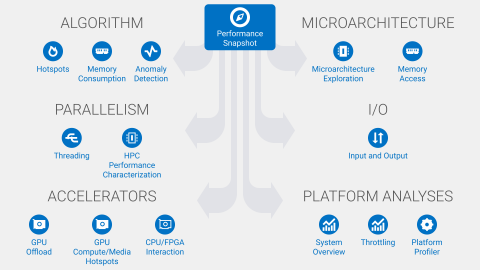
\includegraphics[width=\linewidth]{figures/diagram-vtune-bigpicture-16x9.png}
  \caption{Intel VTune Profiler overview.}
\end{figure}
\end{column}
\end{columns}
\end{frame}

\begin{frame}{Intel Inspector}
\begin{itemize}
  \item Helps find memory errors and nondeterministic threading errors and problems
  \item Dynamic memory and threading error debugger for C, C++, and Fortran applications
\end{itemize}
\end{frame}

\begin{frame}{Intel Trace Analyzer and Collector}
\begin{itemize}
  \item Profiles and analyzes MPI applications
  \item Discover temporal dependencies and bottlenecks
  \item Check the correctness of your application
  \item Locate potential programming errors, buffer overlaps, and deadlocks
  \item Visualize and understand parallel application behavior
  \item Evaluate profiling statistics and load balancing
  \item Analyze performance of subroutines or code blocks
  \item Learn about communication patterns, parameters, and performance data
  \item Identify communication hot spots
  \item Decrease time to solution and increase application efficiency
\end{itemize}
\end{frame}

\section{Further Information}

\begin{frame}{Further Information}
\begin{itemize}
  \item \href{https://www.oneapi.com}{The oneAPI Specification}
  \item \href{https://www.apress.com/gp/book/9781484255735}{Data Parallel C++ (Free eBook)}
  \item \href{https://software.intel.com/content/www/us/en/develop/tools/oneapi/base-toolkit.html}{Intel oneAPI Base Toolkit}
  \item \href{https://software.intel.com/content/www/us/en/develop/tools/oneapi/hpc-toolkit.html}{Intel oneAPI HPC Toolkit}
  \item \href{https://github.com/oneapi-src/oneAPI-samples}{Intel oneAPI Toolkit Samples}
\end{itemize}
\end{frame}

\begin{frame}{Help?}
\centering
Need help or have questions?\\
\href{mailto:rkalescky@smu.edu}{rkalescky@smu.edu} \\
\href{mailto:jlagrone@smu.edu}{jlagrone@smu.edu} \\
\href{mailto:help@smu.edu}{help@smu.edu}  (include HPC in the subject line)
\end{frame}



\end{document}

